\documentclass[a4paper, 12pt, titlepage]{report}

%Taal: Nederlands ("Inhoudsopgave", "Hoofdstuk",...)
\usepackage[dutch]{babel}
\usepackage{graphicx}
\usepackage{subcaption}

%Geen nummering bij secties en hoofdstukkden
\setcounter{secnumdepth}{-1} 

%geen indents
\setlength\parindent{0pt}

\usepackage[dutch]{babel}
\begin{document}

\title{\textbf{Numerieke Modellering en Benadering}\\\textit{Practicum 1: Eigenwaardenproblemen}\\}
\author{De Wolf Peter\\ Vekemans Wout}

\date{\today}
\begin{titlepage}
	\maketitle
	\thispagestyle{empty}
\end{titlepage}

\newpage

\listoffigures

\newpage

\section{Inleiding}
In dit practicum onderzoeken we methoden voor het bepalen van eigenwaarden van vole matrices. In een eerste sectie beschouwen we enkele theoretische eigenschappen van de methoden. In een tweede sectie worden de convergentie-eigenschappen van da methoden onderzocht aan de hand van MATLAB-experimenten. In de derde en laatste sectie gaan we dieper in op \'e\'en van de methoden, namelijk de Jacobi-methode.
\section{Theoretische eigenschappen}

\subsection{Opgave 1}

\subsection{Opgave 2}

\section{Convergentie-experimenten}
Voor al deze experimenten wordt gebruik gemaakt van een volle, re\"ele symmetrische matrix A. We laden hiervoor de gegeven matrix $mat1.txt$ in in MATLAB.

\subsection{Opgave 4}
Het uitvoeren van het $spy$-commando laat zien dat er geen enkel $non-zero$ element in de matrix zit. De uitvoering van het QR-algoritme op een matrix met die afmetingen (nog steeds relatief klein) zou zeer veel werk vragen. \\
Na het reduceren tot Hessenberg vorm zien we dat alle elementen onder de eerste benedendiagonaal nul zijn geworden. Verdere analyse leert ons dat ook de elementen boven de eerste bovendiagonaal allemaal van grootteorde $\epsilon_{mach}$ zijn. Als we de Hessenberg vorm van de matrix afronden tot op 15 decimalen verkijgen we een tridiagonale matrix.(zie figuur \ref{hessenberg}) Dit komt doordat de originele matrix symmetrisch was. De reductie naar Hessenberg vorm zorgt ervoor dat het algoritme niet op een volledige matrix moet inwerken. Het uitvoeren van het QR-algoritme vraagt nu slechts $\mathcal{O}(n^2)$ flops. 
\begin{figure}[!h]
\begin{subfigure}{.5\textwidth}
\centering
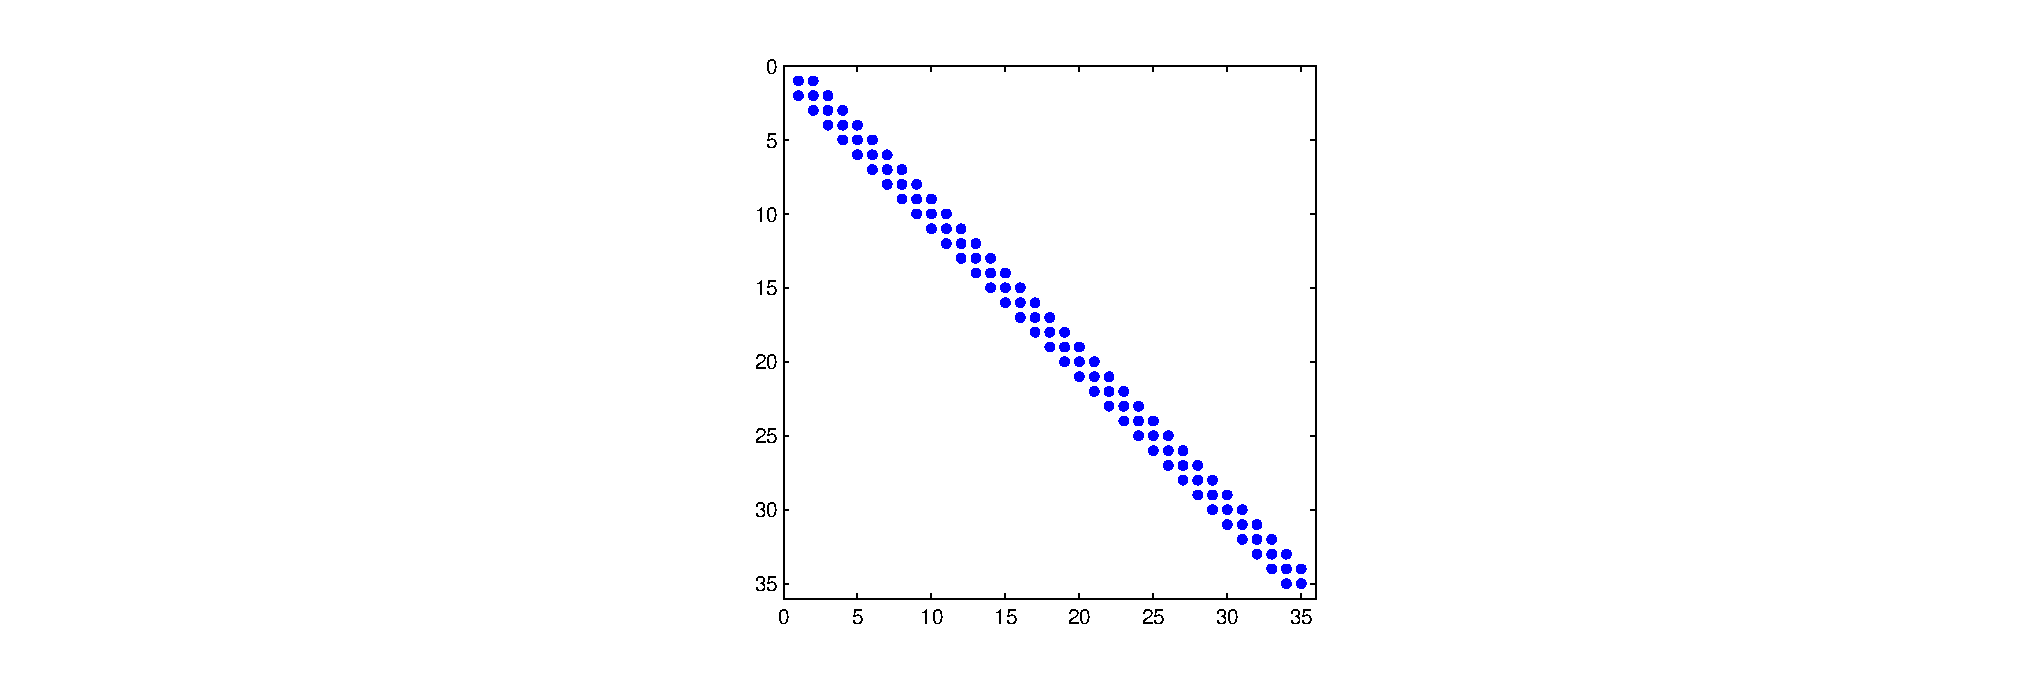
\includegraphics[width=\textwidth]{structuur_hessenberg.eps}
\subcaption{zonder afronden}
\end{subfigure}
\begin{subfigure}{.5\textwidth}
\centering
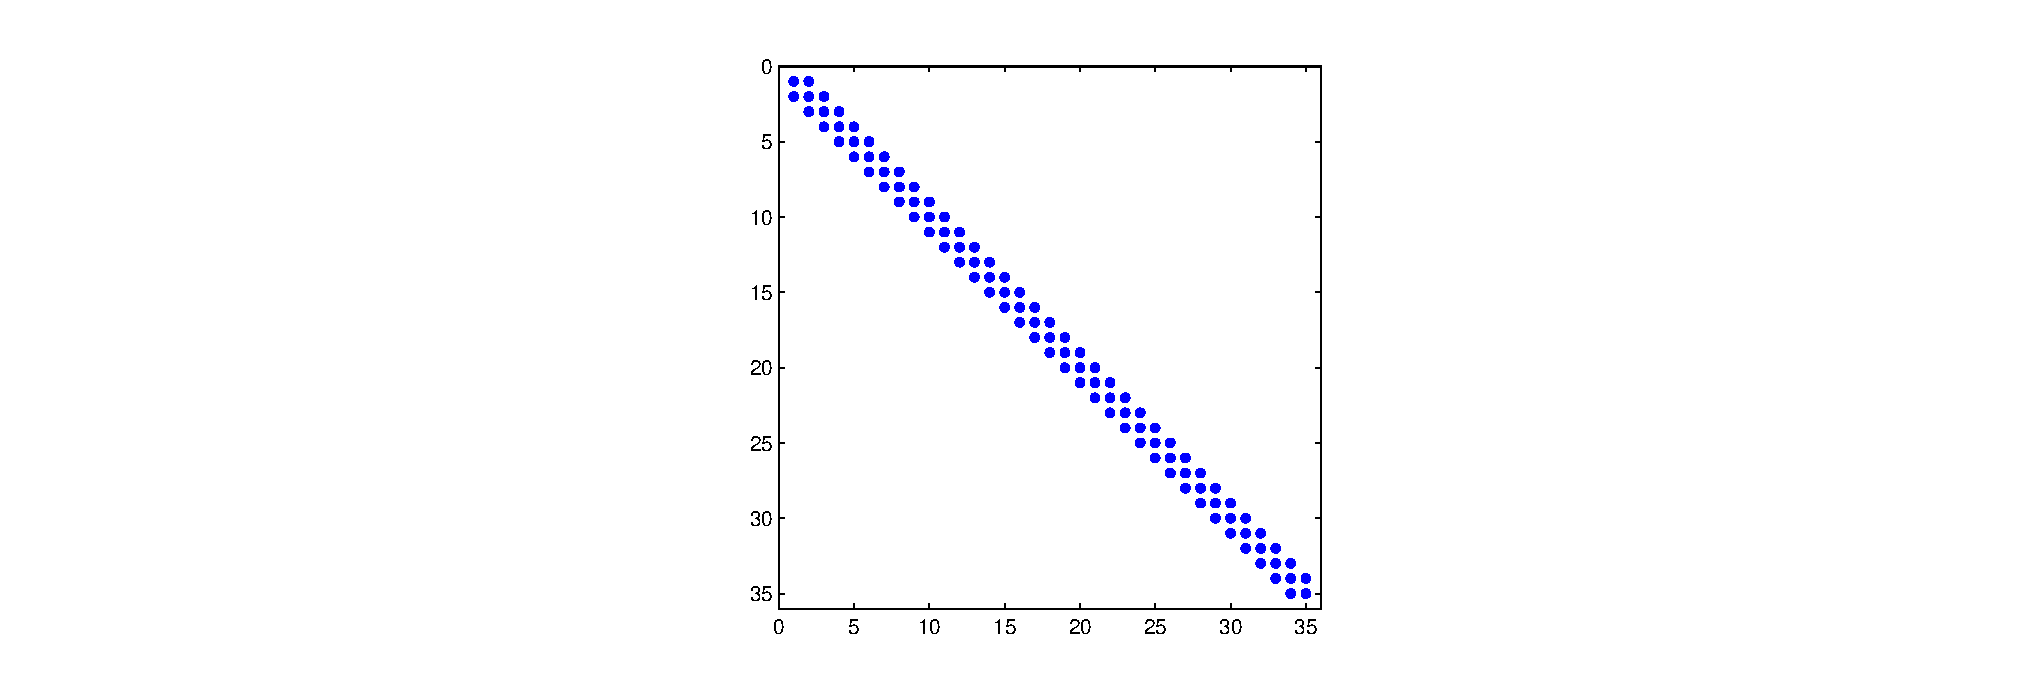
\includegraphics[width=\textwidth]{afgerond.eps}
\subcaption{met afronden}
\end{subfigure}

\caption{Structuur van de Hessenberg matrix}
\label{hessenberg}
\end{figure}

\subsection{Opgave 5}
Na uitvoeren van de drie methoden verkrijgen we ...... TODO we zien duidelijk dat het QR-algoritme zonder shifts een lineaire convergentie heeft. \\

Als residu hebben we het verschil gebruikt tussen de berekende eigenwaarde in elke stap en de re\"ele eigenwaarden. Dit geeft een vrij goed beeld van hoe snel het algoritme
\subsection{Opgave 6}

\subsection{Opgave 7}

\section{Alternatieve eigenwaardenalgoritmen}

\subsection{Opgave 8}

\subsection{Opgave 9}

\subsection{Opgave 10}

\end{document}
